\section{Broader impact and outreach}

The best outreach program should be able to easily reach women and
minority groups underrepresented in science. Video games provide
a good way to do just that- a  study from the  Pew Internet 
\& American Life 
Project (Lenhart 2008) found that the percentage of American youth
that play video games is almost the same for a wide range of racial and
ethnic groups and incomes. The survey covered a
 nationally representative sample of 1,102 young people, ages 12 to 
17. It found that 99\% of boys and 94\% of girls
play video games, and they play them often, with  half of the respondents 
saying they had played a video game the previous day. This adds up to
over 200 million person-hours of video gaming each day in the U.S.

Our proposal 
focuses not on general computer and video games, but on educational games,
and the ideas we incorporate are 
grounded in a theory of intrinsically motivating instruction 
(\cite{Gee03},
\cite{Squire03}, \cite{Schell08}). The documented benefits of gaming
in education have been widely studied, and can be summarized by the 
literature review of \cite{Backlund}. These authors aggregated 40 published
studies on 
gaming's effectiveness in fields varying from Computer Science, 
Language Learning, History, Mathematics, Chemistry and Physics, finding 
overwhelmingly positive outcomes overall, and strong evidence that 
educational games can be effective learning materials in their own right.

The effort will be lead by CMU Physics outreach coordinator Diane 
Turnshek, who has decades of
experience in astronomy outreach to all age ranges, as well
as lecturing undergraduate astronomy at the introductory level.
Other proposal team members will be actively involved. The PI has
experience in educational game design, and will consult with collaborators
in CMU's Entertainment Technology Center, host to several pioneers in 
educational game development. Graduate students will create content
and the undergraduate research students will also play roles
as  classroom mentors and playtesters.




Through the medium of  games, our outreach aims are the following:\\
\noindent {\bf (1a)} To introduce  elementary and middle
school students to the length scales relevant
to astronomy, from the Solar system to the large scale structure of the Universe
.\\
\noindent{\bf (1b)}  To introduce school children to the chemical constituents
 of the Universe and how they are distributed on Astronomical scales.\\
\noindent{\bf (1c)} To introduce high school students to 
 quasars, the  intergalactic medium and absorption lines.\\
{\bf (2)}
To reach the largest audience possible. 
 The gains of this broader 
impact would be to increase interest in science as a career across 
a desirable demographic.

  

\subsection{Minecraft Astronomy lesson plans}




We propose to make lesson plans for elementary and middle school students to 
learn the size scales of the Universe and understand the elemental content 
of the Universe using the popular game Minecraft. 
Minecraft is akin to digital Lego bricks – players inhabit a 
three-dimensional 
world of blocks with its own unique ecosystem and physical laws.
% Using 
%imagination, 
%players build whatever they can dream up by mining resources, combining, 
%and placing them to build everything from pickaxes 
%to complex and working electrical systems. 
So far, 100 million people have 
purchased 
the Mac/PC version of the game. 
It is considered a sandbox game, providing nearly limitless opportunities 
to  build. Teachers can buy discounted licenses through MinecraftEdu.com, as 
well as a plug-in to tailor the software to a specific curriculum. 



\begin{figure}%[ht!]
\centering
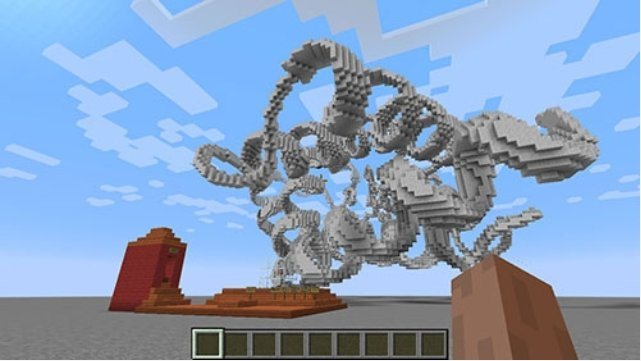
\includegraphics[width=75mm]{figs/myoglobin.jpg}
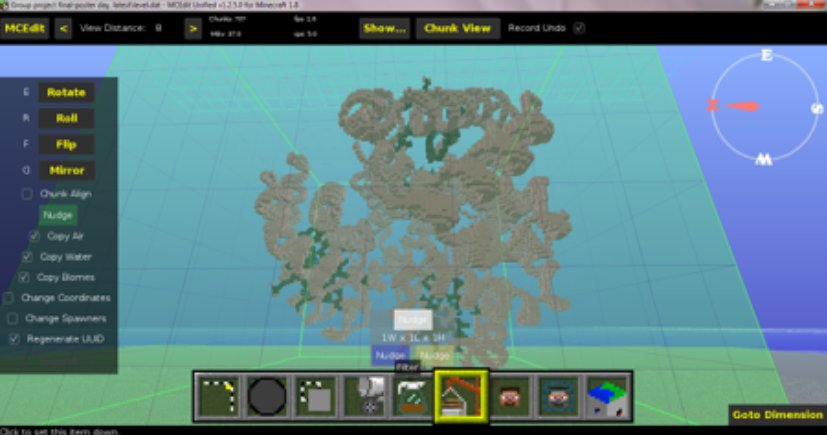
\includegraphics[width=80mm]{figs/mcedit.jpg}
\caption{\footnotesize{{\bf Left:
Minecraft visualization of myoglobin molecule} 
Reproduced from the MolCraft project, University of Hull, UK
{\bf Right: Importing three dimensional structure into Minecraft
using MCedit} Reproduced from the MolCraft project, University of Hull, UK
}}
\label{molcraft}
\end{figure}


As an educational tool, Minecraft teaches design, collaboration,
co-creating and problem solving. It’s an active learning
environment. Previously, successful physics lessons have been created
for studying quantum mechanics (q-Craft Curriculum Project) and
testing gravity (Rhett Alain, Wired) in Minecraft. Gamers enjoy making
maps, building things and solving puzzles.  Our Minecraft Astronomy
elementary school tutorial will give instructions on how to build a
rocket and how to use it to navigate a map of the Universe. 
Our middle school tutorial will include plans to build a
telescope and how to use it to find the atoms that make up our
Universe. Self-driven inquiry leads to locations on our maps where the
content is kept up-to-date.  Blog posts will connect users, guide them
in reflective, “big picture” thought processes, craft intuitive
thinking and inspire their natural curiosity.  Astronomy facts, paired
with math, cosmic pictures and stories will enrich learning.
 
One lesson plan will be primarily for 1st to 4th graders and will
focus on the size scale of the solar system.  We have substantial
experience in this topic as the PI has been carrying outreach to this
demographic since 2002, as part of the CMU Physics department's
outreach program. Some of the outreach activities involved making
scale models of the solar system with household objects.  Several
limitations can be overcome by using the Minecraft world to do this,
including extending the scale of the models arbitrarily, and using the
3rd dimension.  A second lesson plan will focus on the atomic content
of the Universe for middle school students (5th to 7th grade). Game
users will hunt to find the rare metals among the hydrogen and helium
atoms of the universe, finding the prized heavy elements in places
like rocky bodies and supernovae remnants.  We will develop worlds
based on several different length scales, including one where we will
import galaxy redshift survey data (from the SDSS) so that the
students can fly around and explore the large scale structure of the
Universe.  It is simple to import such data sets and edit them- an
example of biological molecules taken from the Molcraft project
(University of Hull, UK) is shown in Figure \ref{molcraft} and it is
easy to imagine how astronomical data would work in this environment.


%Overworld dimensions of the square game plane are $3.59 \times 10^{9}$
% square kilometers 
%(as compared to the Earth’s spherical $5.09 \times 10^{8}$
% square kilometer area). 
%The height  is 256 blocks, but a Sky Dimension of similar size to the 
%Overworld is 
%planned for a future release.

 A shared world will be created and gamer guides 
released to aid exploration. For teachers, lesson plans will be made, 
including  objectives and goals based on educational standards, a 
prior knowledge test, 
directed instruction, vocabulary definitions, guided practice sets and 
an assessment 
worksheet.
The assessments will be crafted to quantify changes in both knowledge 
and motivation to learn (\cite{Rosas03}).
 As our work progresses, we will bring these lessons to a local 
school 
for tests with students.
These include such schools as Colfax School, Milliones School and Helen Faison
academy which we have worked with before, and where there are high fractions
of students from minorities underrepresented in science.
 While these lessons will be available to the 
general public, they will be geared toward educators to be used in classrooms.

\subsection{Universe Sandbox Tutorial}


For high school students, we propose using the commercial software
Universe Sandbox2 (universesandbox.com) to build a Lyman-alpha forest
tutorial and activity.  Universe Sandbox is an interactive space
simulator, giving players the ability t o wander through sections of
the known universe. Universal Sandbox2 is a fully featured, space
simulator, with new features and simulations added based on community
requests. Players have the ability to observe and change the universe
by altering fundamental constants (like the strength of gravity) and
by moving celestial objects through space and time.  Our high school
and introductory college astronomy lesson will walk students through a
Lyman-alpha forest simulation to show intervening material at
differing redshifts. The material creates a forest of absorption lines
and the tutorial will explain how that is seen in the visual in quasar
spectra, using diagrams and an interactive applet that allows the
students to change the density, distance, ionization level and
elemental content of the intervening material. The users discovery
process will be framed as a quest to explain the mystery of changes
the quasar spectrum, as told in comic storyboard form following the
initial discoveries of Martin Schmidt and Cyril Hazard.


Lectures, books, and video are all linear, and linear media are poor at 
conveying complex systems.  The best way to understand a complex 
system is to play with it, getting a holistic sense of how parts are 
connected.  Such systems that are best learned through simulations 
include the human circulatory system and nuclear reactors. 
In physics, demonstrations and laboratories are all simulations, 
traditionally with physical objects, apparatus, and measuring devices.
The Universe itself is the ultimate complex physical system and arguably
the most exciting one to approach in this way.


